%!TEX root = ../thesis.tex
% \title{Kinectograph: Body-Tracking Camera Control for Self-Directed Demonstration Videos}
\chapter{Kinectograph: Body-Tracking Camera Control}
\label{chapter_kinectograph}

A large community of users creates and shares how-to videos online. Many of these videos show demonstrations of physical tasks, such as fixing a machine or demonstrating dance steps. It is often difficult for the authors of these videos to control camera focus, view, and position while performing their tasks.

To help instructors produce videos, in this chapter, we introduce Kinectograph\footnote{This work was published at CHI 2013~\cite{Cheng:2013:BCC:2468356.2468568}.}, a recording device that automatically pans and tilts to follow specific body parts, e.g., hands, of a user in a video with lightweight control. It utilizes a Kinect depth sensor to track skeletal data and adjusts the camera angle via a 2D pan-tilt gimbal mount. Users configure Kinectograph through a tablet application with real-time video preview. We conducted a preliminary evaluations to test the usability of Kinectograph's control interface. All of the participants successfully created instructional videos without assistance. The initial findings suggested that Kinectograph enables instructors to focus on performing their demonstrations, while giving them sufficient camera control at recording time.

%!TEX root = ../thesis.tex
\section{Introduction}

Popular online video-sharing websites such as YouTube have enabled the growth of a large community of users who share their knowledge and expertise in video tutorials. How-To videos demonstrate specific skills and procedures for tasks as varied as cooking, building a treehouse, or fixing a machine \cite{Torrey:2007he}.
These online tutorials help learners observe the manipulations and then put them into practice \cite{Torrey:2009fc}. However, in recording these videos, instructors often find it challenging to control the camera during demonstration.
%
Working with a cameraman who controls the device and viewpoints ensures that the video captures the movements that the audience would want to see, but it requires having a second person to direct the recording and work closely together with instructors. Many amateur users who mostly work alone, therefore, choose to self-record with one or more cameras. Camcorders can be set on a tripod to capture a static viewpoint, but it is hard to make sure whether users' actions are properly in frame at recording time. An alternative is to wear a head mounted camera to record what the instructors see. This may record unwanted and distractive head movements, making it difficult for the audience to watch. Additional camera views of the overall workspace might be needed to assist learners with understanding the context of demonstrated actions \cite{Fussell:2003te}.

\begin{figure}[t]
\centering
\vspace{0.15in}
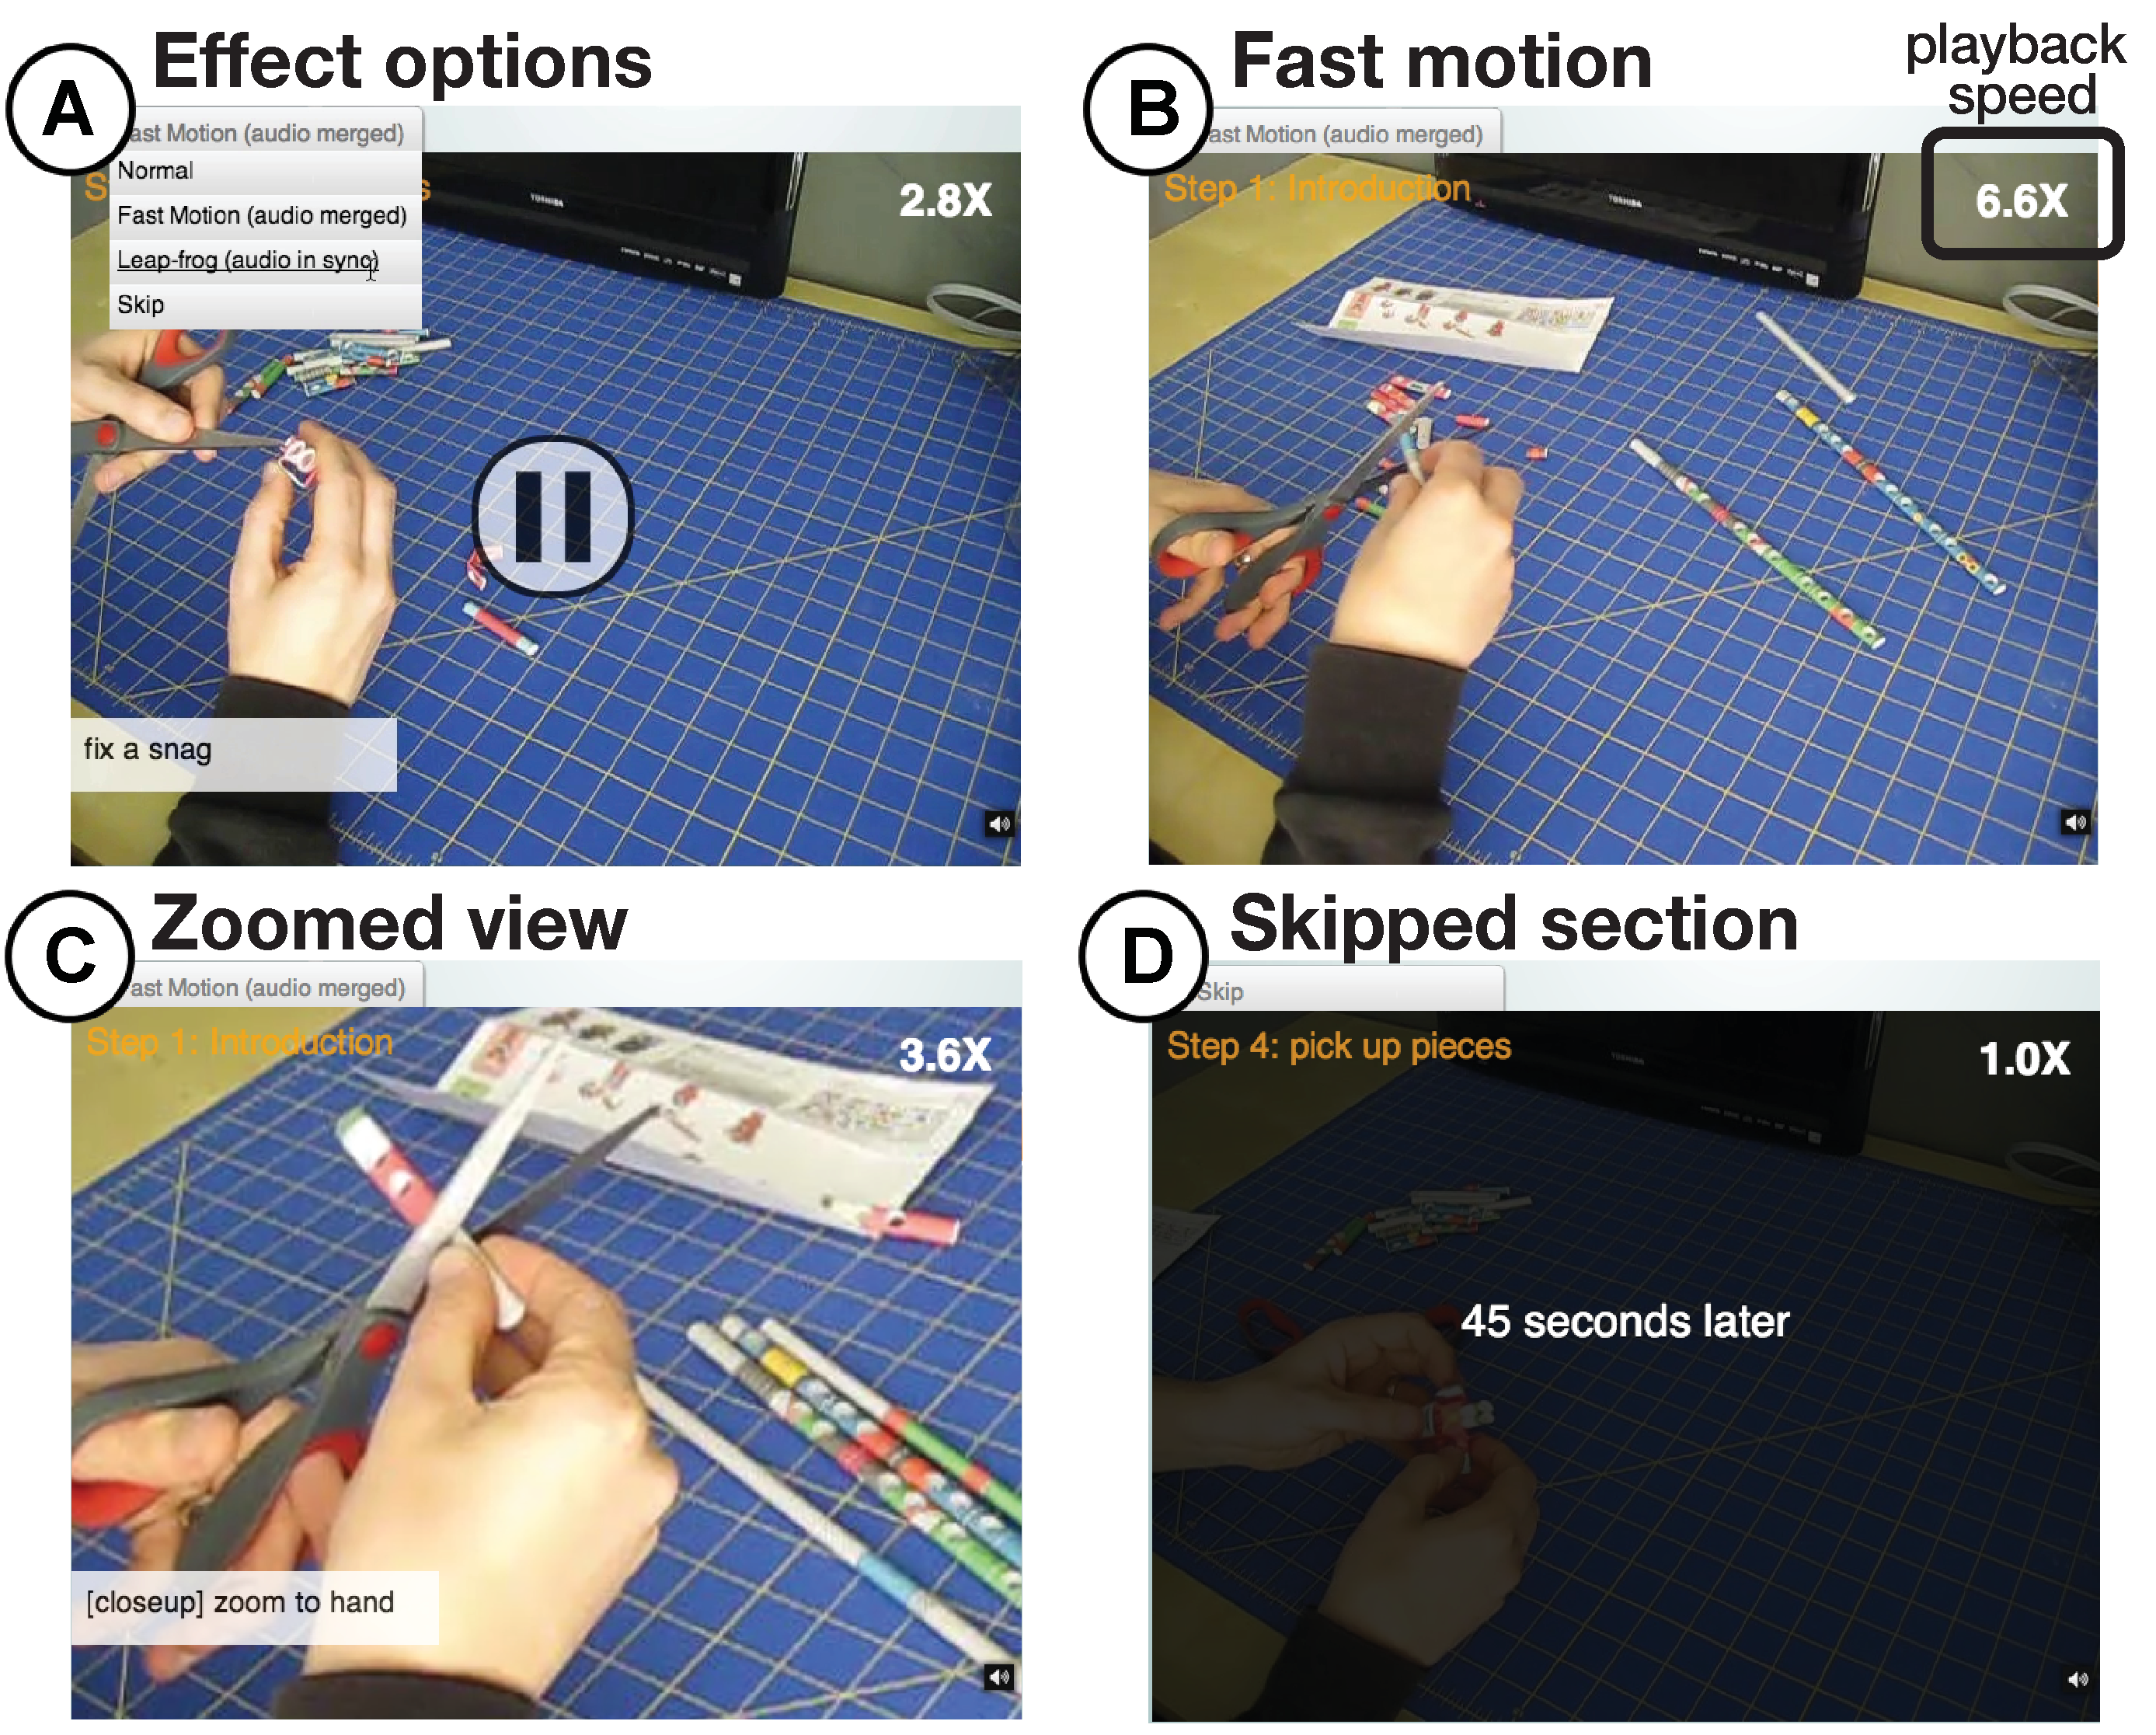
\includegraphics[width=1.0\columnwidth]{\kinectograph/fig/teaser.pdf}
\caption{Kinectograph includes a Kinect camera to track user movement and a motorized dock to pan and tilt the camera so that the user (or their hand) remains centered in the recorded video. Here the device follows the user\'s hand while he is illustrating.}
\label{fig:figure1}
\end{figure}

Seeing these filming challenges, we would like to enable users to gain the flexibility of real-time camera control without requiring a dedicated camera-person. Our goal is to design a device that can automatically track and orient to film the tutorial instructors while providing lightweight manual controls. Existing video conferencing cameras and surveillance tools offer human tracking to provide full or partial automatic viewpoint control. Polycom\footnote{http://www.polycom.com/} designs video conferencing cameras that feature face recognition and voice detection to enable a group of users to talk in an office room setting. This approach assumes people's faces should be in the frame, which may not be true for instructional videos that focus on actions rather than ``talking heads.''
%
Automatic motion tracking is possible to always keep the user in view using visible markers \cite{Ranjan:2010} or wearable sensors such as infrared emitters by Swivl\footnote{http://www.swivl.com/}. However, instructors are unlikely to take such approaches to put on visible markers when demonstrating.
%
Researchers have been developing techniques to track specific targets using computer vision, including hands \cite{Ranjan:2008}, user movements \cite{Wilson:2012fb}, fast-moving objects (e.g., a Ping-Pong ball) \cite{Okumura:2011tr}, or regions in pre-defined spaces \cite{Ranjan:2007}. These usually require an expert defining heuristics of space regions or movement classifications ahead of time for the tracking program. On the contrary, we aim at proposing a new approach that does not have these issues, gives users flexibility in a home environment, and provides interactive control over the behavior of the camera tracking.
%
% TeleAdvisor assists a helper to remotely observe a physical task in real-time and provide instructions~\cite{Gurevich:2012ko}. However, the system is limited by the static camera view without automatic tracking.
%

We propose Kinectograph, a new device that enables semi-automatic camera control for users to self-direct camera orientation for demonstration tasks (Figure~\ref{fig:figure1}). Kinectograph serves as both the camera and the cameraman. It provides a motorized dock for a Kinect\footnote{http://www.xbox.com/en-US/kinect} sensor and a tablet-based user interface (separate from the camera) to switch between tracking regions at runtime based on their needs when demonstrating. Using skeleton tracking to follow the user’s movement, Kinectograph automatically pans and tilts the camera in real time. Users can define zoom regions that follow his actions to provide closeup views. Using a Kinect sensor, our system works in a common indoor setting and does not require the user to wear sensors or configure the environments. Kinectograph makes a novel contribution over the prior art in its mixed-initiative approach that offers various levels of automation and control to users at record time.

In this paper, we describe the user experience of recording with Kinectograph. We also describe design and implementation decisions. Finally, we review findings from a preliminary evaluation with 7 participants to study Kinectograph's usability of self-recording tutorials. All of the participants successfully created a demonstration video using our system without assistance and found it easy to interact with.

%\bjoern{I cut this out because you are missing the reference.}\new{In [insert citation here], they similarly use motors and a camera to automatically track and zooming in on users, but they do so in a conference setting. One of their system objectives is to unobtrusively track; however, our system focuses on providing enabling user's control in these tracking and zooming decisions for their DIY tutorials. In addition they only use facial and audio tracking and do not leverage the power of the kinect to do skeletal tracking.}

% Abhishek Ranjan, Jeremy Birnholtz, Rorik Henrikson, Ravin Balakrishnan, Dana Lee. (2010). Automatic camera control using unobtrusive vision and audio tracking. Proceedings of GI 2010 – the Graphics Interface Conference. p. 47-54.
%\pc{Where is the reference to the papers Bjoern sent? auto-tracking camera}


%!TEX root = ../thesis.tex
\section{Recording Video Tutorials with Kinectograph}
\label{kinectograph_authoring}

\begin{figure}[t]
\centering
\includegraphics[width=0.7\columnwidth]{\kinectograph/fig/newui}
\caption{Kinectograph UI on a tablet device.}
\label{fig:figure4}
\end{figure}

Users connect the Kinectograph device to a personal computer and start its server software, then open the Kinectograph mobile control UI (Figure \ref{fig:figure4}) on a phone or tablet that they can carry with them during their demonstration.
%
In order to allow How-To tutorial makers as much control over the filming of their tutorial with as little effort as possible, Kinectograph offers the following features on its mobile control UI:

\subsection{Real-time Video View}
In a self video recording, it is convenient for the user to be able to view the current state of their video to make filming decisions. Thus, Kinectograph's UI displays a real-time video feed (currently limited to a low fps) from the Kinect camera.

\subsection{Manual Control}
Users can manually control the camera angle by swiping on the preview image to pan and tilt the camera. For example, during a cooking demonstration, users may wish to pan to a shot of the oven to their left or the sink to their right, or tilt down when they open the oven.

\subsection{Automated Tracking Control}
Demonstrations may require users to move around, such as in furniture assembling or personal training videos. Kinectograph's automated tracking control enables users to focus on their demonstration. Thus, users can switch to automatic camera mode to have Kinectograph track them. Kinectograph can follow one or two actors. Users select which body parts should remain in the frame by tapping on targets of an iconic body outline in the UI - e.g., the head (as in video conferencing systems) or the hands (which may be more important for demonstrations). To keep the entire upper body in view, users can select multiple joints simultaneously. Each selected joint can be deselected by toggling the target button on the iconic body outline.

Early testing showed that because the video feed to the tablet has some latency and a lower framerate, selecting joints on the video feed itself can be difficult if those joints are moving. We therefore chose to display a static, iconic body outline.
%display an iconic body outline next to the video feed on the UI to give users a static target for activating and deactivating joint tracking.

\subsection{Zoom Control}
Close-ups of important steps are a common editing technique in demonstration videos. To capture close-ups, users can define a zoom region related to their body by dragging a rectangular area across the iconic body outline - e.g., they can draw a region that captures their hands to focus on their hand motions. Because the camera used has a fixed focal length, our current prototype uses digital zoom (Figure~\ref{fig:ZoomView}). By default any joints in the zoomed region are automatically added to the track list.

\subsection{Reset}
Finally, the control UI provides a button to dismiss any joints selected for automated tracking or for target zooming.

\begin{figure}[t]
\centering
\includegraphics[width=0.6\columnwidth]{\kinectograph/fig/ZoomView}
\caption{Kinectograph tracks and provides a digital zoom view (right) captured from the Kinect camera view (left) in real-time based on user specified area.}
\label{fig:ZoomView}
\end{figure}

\begin{figure}[t]
\centering
\includegraphics[width=0.7\columnwidth]{\kinectograph/fig/arch.png}
\caption{Kinectograph architecture.}
\label{fig:architecture}
\end{figure}


%!TEX root = ../thesis.tex
\section{Automatic Tracking Techniques}
Kinectograph streams the video view captured from a Kinect camera to a PC. This PC also acts as a web server, publishing the control interface to tablet or phone clients. When a user enables automatic tracking, the PC analyzes user movements using the skeletal data from the Kinect SDK. Based on the user position, it sends appropriate commands to the motorized dock via USB to move the camera (Figure~\ref{fig:architecture}).

\subsection{Hardware}
To control the camera view, Kinectograph utilizes the motor system and base provided by the Kubi\footnote{http://www.revolverobotics.com/}, a dynamic telepresence solution for video calls. This connects to the Kinect with a 3D printed holder (Figure~\ref{fig:figure1}). The Kubi uses two Dynamixel AX-12 motors\footnote{http://www.crustcrawler.com/motors/AX12/index.php}, to pan and tilt. Instead of using Kubi's motor control API and microcontroller, we connect Kubi's motors to an external Arduino Mega (ATmega1280)\footnote{http://arduino.cc/en/Main/arduinoBoardMega} so we can better customize the control of the Dynamixel motors.
% To control the camera view, we designed a specialized dock that holds the Kinect sensor and that can be rotated using a pan-and-tilt servo kit in two axes (Figure~\ref{fig:device}). A bottom servo moves the Kinect left and right (180 degrees), while the top servo moves it up and down (90 degrees from horizon in order to capture the user working area). The mount allows full 180-degree rotation for both horizontal and vertical axis. To control the servo motors of the pan-tilt mechanism, an embedded microcontroller (8-bit ATmega32U4) generates PWM (Pulse-Width Modulation) signals. A base, fabricated on a Projet HD 3000 printer, stabilizes the system and houses the electronics.

%The bottom servo of the pan-tilt system fastens to the middle of the base, while the Kinect holder attaches the Kinect to the pan-tilt system .

% \begin{figure}[t]
% \centering
% \includegraphics[width=0.7\columnwidth]{device-annotated.jpg}
% \caption{The Kinectograph device combines a depth camera and a robotic pan-tilt mount.}
% \label{fig:device}
% \end{figure}

\subsection{Auto-Tracking Algorithm}

\subsubsection{Motion Tracking and Servo Adjustment}
To track the user position and determine the camera angle, our system analyzes the skeletal tracking data and depth information of a user’s body parts received from the Kinect sensor in real-time. Using Kinect enables the user to freely move or turn around, with support of self-occlusion \cite{Shotton:2011ud}. Currently Kinectograph tracks one or two people. If more people are present, only the two closest are tracked.

\subsubsection{Physical Tracking of Joints}
Kinectograph angles the camera to position the target, such as a user's hand, in the center of the camera view. When a user is found in the view, it receives the position of the tracked joint located at $\textless pos_{x}$, $pos_{y}$, $pos_{z} \textgreater$ in the 3D space that represents a {\em x-y} coordinate and {\em z} as the depth information of the target. The rotation angles are computed in order to align the target joint to the position of the center of view at $\textless center_{x}$, $center_{y}$, $pos_{z}\textgreater$  on the same X-Y plane as the joint position. The rotation angles $\theta_{tilt}$ and $\theta_{pan}$ (in degrees) to tilt or pan the camera are:

Tilt angle of y-axis:
% Θ_tilt=∆y/∆z=arctan⁡((center_y-pos_y)/(pos_z ))
$\theta_{tilt}=\frac{\Delta y}{\Delta z}=\arctan{(\frac{center_{y}-pos_{y}}{pos_{z}})}$

Pan angle of x-axis:
% ∆Θ_pan=∆x/∆z=arctan⁡((center_x-pos_x)/(pos_z ))
$\theta_{pan}=\frac{\Delta x}{\Delta z}=\arctan{(\frac{center_{x}-pos_{x}}{pos_{z}})}$

Figure \ref{fig:math} depicts the geometric relations from the Kinectograph view. Every 10 ms the top motor turns by $\theta_{tilt}$ and the bottom motor turns by $\theta_{pan}$. To avoid extraneous small camera movements, a variable bounding box around the center of the field of view is set such that the Kinectograph only moves once the tracked object leaves the bounding box.

% Our current Kinectograph prototype limits users to selecting only joints in the upper portion of their body. Tracking joints such as the feet may cause the parts of the user to be out of the Kinect camera's view and thus be difficult to recognize. More sophisticated techniques may take into account the distance of the user and the availability of other joints in order to decide when it would be appropriate to track such joints. %For example, allow users to only track the feet, Kinectograph is confident that this would not cause the user to be unrecognizable.

% \subsubsection{Tracking Multiple Joints and Multiple Actors}
To support multiple target selection, we use the same $\theta_{tilt}$ and $\theta_{pan}$ formulas as above, except $\textless pos_{x}$, $pos_{y}$, $pos_{z} \textgreater$ represents the average of all tracked joint positions rather than the position of one tracked joint.
%
% Given...we can move the camera to position multiple targets (i.e. multiple body joints)
If there is more than one actor in the view, users can select joints from the second user. All selected joints are treated equally to be tracked, and thus the camera angle adjustment works as it does in the previous multiple-joint scenario.

%This method was used for Kinectograph's first prototype for simplicity reasons, with knowledge that their would be limitations. We discuss these limitations farther in our Second User Study section.
% add notes about limitations somewhere else down there about wide anglea nd
% smarter tracking physical limitation

\begin{figure}[t]
\centering
\includegraphics[width=1.0\columnwidth]{\kinectograph/fig/MathFinal}
\caption{Kinectograph tracks the position of the target (A) and computes the tilt (B) and the pan (C) angles in order to center the target. It digitally zooms the camera view based on user specified region on the Tablet UI (D).}
\label{fig:math}
\end{figure}

\subsubsection{Digital Tracking and Zooming}
% \bh{The Kinect has fixed field of view so we perform digital zoom. This is valuable in demonstration videos to direct the viewer's attention. For higher resolution zooming, future hardware embodiments could either employ a camera with programmable region-of-interest on the sensor, or a camera with a programmatically controllable zoom lens.}

% \bh{Describe how you zoom in initially; when you decide to zoom out, and why you made these decisions.}
Users may find it important not only to center a joint in the view but also magnify it, such as zooming into the hand during a demonstration showing how to stir the ingredients.
%
Thus, Kinectograph allows users to digitally zoom into a specific area with one or more joints. Our algorithm attempts to keep the joint(s) in the same relative position as it was in its initial zoomed in view. This feature works independently of the physical tracking and thus does not require physically controlling the motors or camera.
%
Kinectograph allows the the user to draw a box on the figure in the UI around the joint she wishes to digitally track. The initial dimensions and positions of that translated zoomed region on the live video stream is determined as follows (Figure~\ref{fig:math}D), where:

$ZoomWidth= R + L = \frac{W}{2}*\frac{l}{\frac{w}{2}} + \frac{W}{2}*\frac{r}{\frac{w}{2}}$ \\
$ZoomHeight= U + D = \frac{H}{2}*\frac{u}{\frac{h}{2}}+ \frac{H}{2}*\frac{d}{\frac{h}{2}}$

After the zoomed region's initial dimension has been set, the center of this region is continuously shifted using the following equations: $\Delta X = pos_{x}^{'}-pos_{x}$ and $\Delta Y = pos_{y}^{'}-pos_{y}$

% \begin{figure}[t]
% \centering
% \includegraphics[width=1.0\columnwidth]{Zoom}
% \caption{Describes the the initial dimensional sizing of the zoom region}
% \label{fig:zoom}
% \end{figure}


%!TEX root = ../thesis.tex
\subsection{Implementation}
The video and audio analysis is implemented in Matlab. The Annotation and Editing Interfaces are implemented with standard Web technologies (HTML5, CSS3, and JavaScript). An Apache web server hosts these web pages and sends the user annotations to the back-end Matlab system.
%Once the video is processed, the server updates the video rendered with generated metadata on the web interface. When user modified the automatic effects and text annotation in real-time, DemoCut records the changes and updates the metadata for outputs.


%!TEX root = ../thesis.tex
\section{Evaluation}
\label{kinectograph_study}

This section presents user feedback collected from three preliminary studies that we conducted to answer questions: What activities would users find useful to capture using Kinectograph? How well could users create self-directed tutorials with Kinectograph?

\subsection{Study 1: Demo at an Expo}
We demonstrated an initial design of Kinectograph (see Appendix C) at a public exhibition to approximately 60 people. Each participant was allowed to enter our capturing space and experience the device. Based on our observation and conversations collected, we found that people were convinced by the idea as soon as they walked into the scene when Kinectograph started to move along. These questions were often asked: \iquote{How fast was Kinectograph able to follow me?} and \iquote{Can I switch to track other parts (like my hand)?}. With the tablet device control, participants soon were successful in controlling the camera. They often walked, ran, and danced to test the tracking. We also learned that people expected the device to provide fast response in various conditions such as turning, rapid change of directions, or partial occlusions (when people were hidden by furniture or large objects).

\subsection{Study 2: Test on Recording Activities}
To understand how Kinectograph can support users in demonstrations, we invited four participants (3 male and 1 female, aged 22-29) who did not join the exhibition to our user study in a home environment. We aimed to explore whether users prefer to watch the video captured by Kinectograph over video recorded with a static camera, and whether Kinectograph can capture complete demonstrations
 that a static camera cannot achieve.

We first introduced Kinectograph by having participants walk around while the device tracked. We encouraged participants to brainstorm some activities they wanted to record. Once the task was decided, they were asked to set up both a static camera and the Kinectograph with our tablet device and start the recording. There was no time constraint during the study. A short post interview was then conducted, in which we showed the recorded videos from both cameras on a PC.

\begin{table}[b!]
     \centering
    \includegraphics[width=1\columnwidth]{\kinectograph/fig/study2}
    \caption{Task information and results collected in the preliminary user study.}
    \label{tab:kinectograph_first_tasks}
 \end{table}

\begin{figure}[t!]
     \centering
    \includegraphics[width=0.5\columnwidth]{\kinectograph/fig/OurExamples-2x2}
    \caption{Examples of camera views captured by a static camera and Kinectograph at two specific moments in time.}
    \label{fig:kinectograph_dance}
\end{figure}

Table~\ref{tab:kinectograph_first_tasks} shows details of the four tasks and analysis of the recorded videos. We categorized physical activities into three movement types: \emph{Continuous} (user continuously moves around), \emph{Periodic} (user moves, stays, and moves again periodically), and \emph{Occasional} (no clear motion pattern was observed).
%
There were two Continuous and two Periodic tasks that participants designed. The moving range was about 15 feet in a home environment, and participants set the static camera about 8 feet away from the center of their workspace. Participants chose this distance to avoid out-of-frame problems with the static camera: \iquote{The distance was chosen so that all of the activity could be captured} (P4). Kinectograph was placed 6 feet away on a tabletop by the experimenters to capture the participant's whole body. Participants were allowed to adjust the camera angle via our tablet UI before recording the demonstration.

All the participants chose to track their heads, but note
that their activities involved frequent turning where
pure face recognition might fail. Participants did not
change this setting during the performance, although
they were allowed to. P2 changed to the manual mode
for testing, switched back, and then continued the
activity. The average video length is one and half
minutes long.

All the participants agreed or strongly agreed that
Kinectograph captured what they intended to show,
while only half of them agreed that the static camera
captured as expected. The main reason was the
limited static camera angle; in three tasks, participants
moved out of the static camera view more than once
. Figure~\ref{fig:kinectograph_dance} shows two examples where our system
captured what the static camera missed. It was worth
noting that although P3 had set and confirmed the
viewpoint before recording, he was not aware that he
shortly but frequently (9 times) went over the
boundaries when he was demonstrating. He explained
that he preferred using Kinectograph because it \iquote{kept
us in the center of view no matter how we moved
around.} This shows that Kinectograph successfully
ensured the activities would be captured and therefore
enabled users to focus on their tasks.

\subsection{Study 3: Self-Recording Activities}

Finally, we conducted a study to measure whether users could film an entire demonstration video using Kinectograph with minimal aid.
%
We recruited seven participants (3 male and 4 females, ages 20-33) from a university to record multi-step tutorials in a lab environment. Four had filmed a video before but only one had filmed a video without the assistance of others. Each participant was compensated with a \$10 giftcard. Each session lasted about 30 minutes long.
% Note that this experiment was run using a previous prototype of the Kinectograph base, which did not utilize the motors provided by the Kubi.
%\pc{describe the settings and put the figure here}
%14-16 feet by 12-14 feet area

\subsubsection{Procedure and Tasks}
\subsubTitleBold{Introduction (5 minutes)} Participants first went through an online documentation to learn the Kinectograph features. %with a demo video

\subsubTitleBold{Training (10 minutes)} Experimenters guided participants through a series of interactions highlighting each of our core features. Participants were asked to operate each feature through our Tablet UI with the support of experimenters.

\subsubTitleBold{Testing (5 minutes)} We asked participants to film a basketball tutorial using Kinectograph. They were asked to introduce actions including passing, catching, and tossing a basketball. Participants acted as both an actor and a director, i.e., they fully controlled the camera and performed the demonstrations without any assistance. A series of nine subtasks were designed for participants to exercise the following features: manual mode (pan/tilt), tracking mode (to track single and multiple body joints), and zooming. In particular, one of the subtasks involved two users in the view. Experimenter walked in the view for passing the ball when participant invited. To help participants understand these activities, we provided a storyboard with high level instructions for filming (e.g., ``zoom into your face'', ``pan to the basketball'', or ``track your head and walk around'') without explicitly listing which Kinectograph feature to use. During the recording, we captured Kinectograph's rendered video view.

\subsubTitleBold{Questionnaire and Debrief (10 minutes)} Finally, we asked participants to watch the recorded video in full and answer a questionnaire, regarding the ease of use of our interface and open-ended questions. We monitored the number of attempts it took to complete each filming task of the tutorials.

\subsubsection{Results}
% \subsubsection{Successes}
All of the 7 participants successfully created a self-directed tutorial using our system. No users failed to complete any of the 9 subtasks. Each participant reattempted at most 2 subtasks, mostly to reselect a zoom area. The average video length was 3.5 minutes. Overall, participants rated the ease of use of the system as $\mu=4.1$ on the 5-point Likert scale.
%
All participants were able to manually pan and tilt the camera by swiping as intended. Participants stated that this was easy to control with the UI ($\mu=3.6$ , $\sigma = 1.0$). They also successfully enabled the tracking mode and had Kinectograph track their head and hands. Participants stated it was easy to enable tracking ($\mu=4, \sigma=1.3$ ) and rated their satisfaction with the system performance as $\mu=4, \sigma=0.8$.  Participants stated that \iquote{It was easy to select a body part of choice} (P6), and that \iquote{ (...Kinectograph) could center the screen very well, and accurately tracked the person} (P7). Four users specifically mentioned that zooming was one of the features that worked well. Participants were satisfied with their video recording ($\mu=4.1$, $\sigma=0.7$).

%{\bf Reset} All participants were able to complete the reset task in one try. unimportant

% \subsubsection{Shortcomings}
We also learned some important shortcomings from the study. Notably, the pan-tilt motors that our previous Kinectograph prototype uses is under-dimensioned, which leads to oscillation (camera shake) when Kinectograph performs large amplitude pan movements. This is less noticeable at further distances, but becomes especially problematic when the users zooms in on small regions. Learning this effect, we have removed this issue with our current use of Kubi's servos, which provide smooth motor control.

Latency in video streaming to the tablet device hampered usability. As P4 stated: \iquote{The lag made it difficult for me to move the kinectograph smoothly [during manual control]}.
%
% Tracking multiple actors remained somewhat difficult (a confederate joined for a ball passing task). P1 stated \iquote{Shortcomings were only really with multiple people in the demo, and the limitations of the viewing angle of the Kinect itself.}
%
Participants also suggested alternative control modes other than a tablet while engaged in bi-manual tasks: \iquote{Certain demos require the use of multiple hands, meaning that I can't carry the iPad during the demo if i wanted to change the point of focus on my body. It would be nice if there were gestures i could do to switch the point(s) of focus without having to use the iPad.} We found this concept interesting and plan to explore in future work.

% \begin{figure}[t]
% \centering
% \includegraphics[width=1.0\columnwidth]{userStudy}
% \caption{We presented participants in the second procedure with a storyboard of actions they should perform.}
% \label{fig:storyboard}
% \end{figure}
% In aggregate, our evaluation suggests that Kinectograph system is capable of being used to create tutorial videos but also points the way for future work. Future work comprises improvements to live video streaming, better support of multiple users (i.e. using voice commands or gesture cues to control), and using kinectic info and zoom as meta data for playback. \dc{add more?}


% and more Tablet UI features, such as picture in picture view and more boxes on the UI to provide further feedback to the user.


\section{Conclusion}
We presented Kinectograph, a new device that provides automatic and user-controlled camera orientation. We showed initial evidence of its effectiveness for self-recording demonstration tasks. We see applications of Kinectograph beyond the domain of instructional video and are investigating the opportunities of rich tracking information for video recording and editing in general.

%\section{Note on prior submission}
%This paper is based on a non-archival poster accepted for publication at CHI 2013. The prior version used a substantially different user interface and %backend. We also expanded the evaluation of our system in this submission.

% and whether the user's actions with the UI produced the expected result. we aimed to confirm that our features did work well and that the UI was easy enough to use to perform an assigned task.}

% Balancing columns in a ref list is a bit of a pain because you
% either use a hack like flushend or balance, or manually insert
% a column break.  http://www.tex.ac.uk/cgi-bin/texfaq2html?label=balance
% multicols doesn't work because we're already in two-column mode,
% and flushend isn't awesome, so I choose balance.  See this
% for more info: http://cs.brown.edu/system/software/latex/doc/balance.pdf
%
% Note that in a perfect world balance wants to be in the first
% column of the last page.
%
% If balance doesn't work for you, you can remove that and
% hard-code a column break into the bbl file right before you
% submit:
%
% http://stackoverflow.com/questions/2149854/how-to-manually-equalize-columns-
% in-an-ieee-paper-if-using-bibtex
%
% Or, just remove \balance and give up on balancing the last page.
%
